\documentclass{beamer}
\usepackage[latin1]{inputenc}
\usepackage{bm}
\usetheme{Warsaw}
\title{Introduction to Nuclear Magnetic Resonance Spectroscopy}
\author{Dr Alexey Potapov}
\institute{University of Nottingham, School of Physics and Astronomy}
\date{Jule 13, 2017}

\setbeamertemplate{headline}{}
\setbeamertemplate{footline}{}
\setbeamertemplate{caption}{Fig.\insertcaptionnumber: \insertcaption \par}
\setbeamerfont{caption}{size=\scriptsize }
\setbeamercovered{invisible}
\setbeamercovered{%
	again covered={\opaqueness<1->{50}}}
%\newenvironment{slide}[1]
%{\begin{frame}[environment=slide]
%		\frametitle{\insertsection-#1}}
%	{\end{frame}}


\begin{document}
	
	\begin{frame}
		\titlepage
	\end{frame}
	
	\section{Introduction. Magnetic moment in magnetic field.}
	\subsection{Introduction to Magnetic Resonance}	
	\begin{frame}{\thesection.\thesubsection. \insertsubsection}

		
		\begin{itemize}
		\item Magnetic resonance (MR) is a phenomenon of resonant energy absorption by a system of nuclei (and electrons). 
		\item Nuclear magnetic resonance (NMR) results from the intrinsic magnetic moment of the
		nuclei of some atoms. Magnetic moments of electrons are exploited in electron spin resonance.
		\item Magnetic resonance (MR) generally involves placing a sample in a strong magnetic
		field (to generate polarisation at a fixed resonant frequency) and detecting signals
		produced following application of pulsed radio-frequency electromagnetic fields (RF
		pulses).
		\item MR is a very powerful method for studying the structure of materials: used in physics, chemistry, biology, medicine etc.

		\end{itemize}
	\end{frame}
	
	\subsection{Applications of NMR}
	
	  	
	
	\begin{frame}{\thesection.\thesubsection. \insertsubsection}
	
	 \begin{itemize}
	 	\item NMR spectroscopy is used for chemical analysis and for molecular structure determination	  	
	 \end{itemize}
	 
	
		
		\begin{figure}[ht]
			\begin{minipage}[t]{0.45\linewidth}
				\centering
				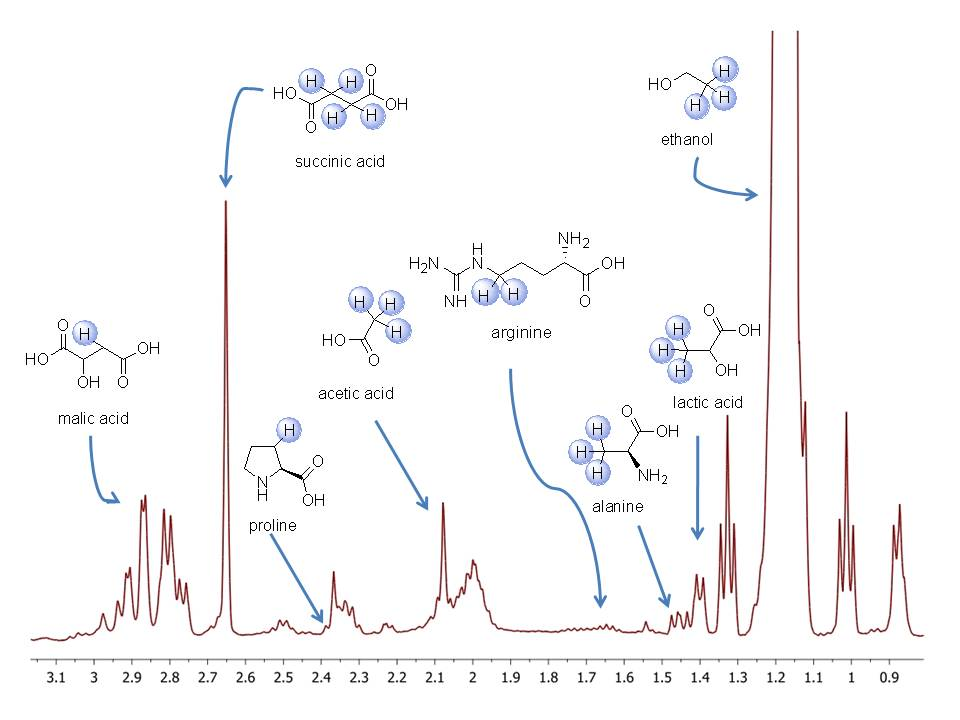
\includegraphics[width=\textwidth]{wine_spectrum.jpg}
				\caption{\textsuperscript{1}H NMR spectrum of a sample of Spanish wine (\url{http://www.unirioja.es/gsoe/NMR.htm})}
				\label{fig1}
			\end{minipage}
			\hspace{0.3cm}
			\begin{minipage}[t]{0.45\linewidth}
				\centering
				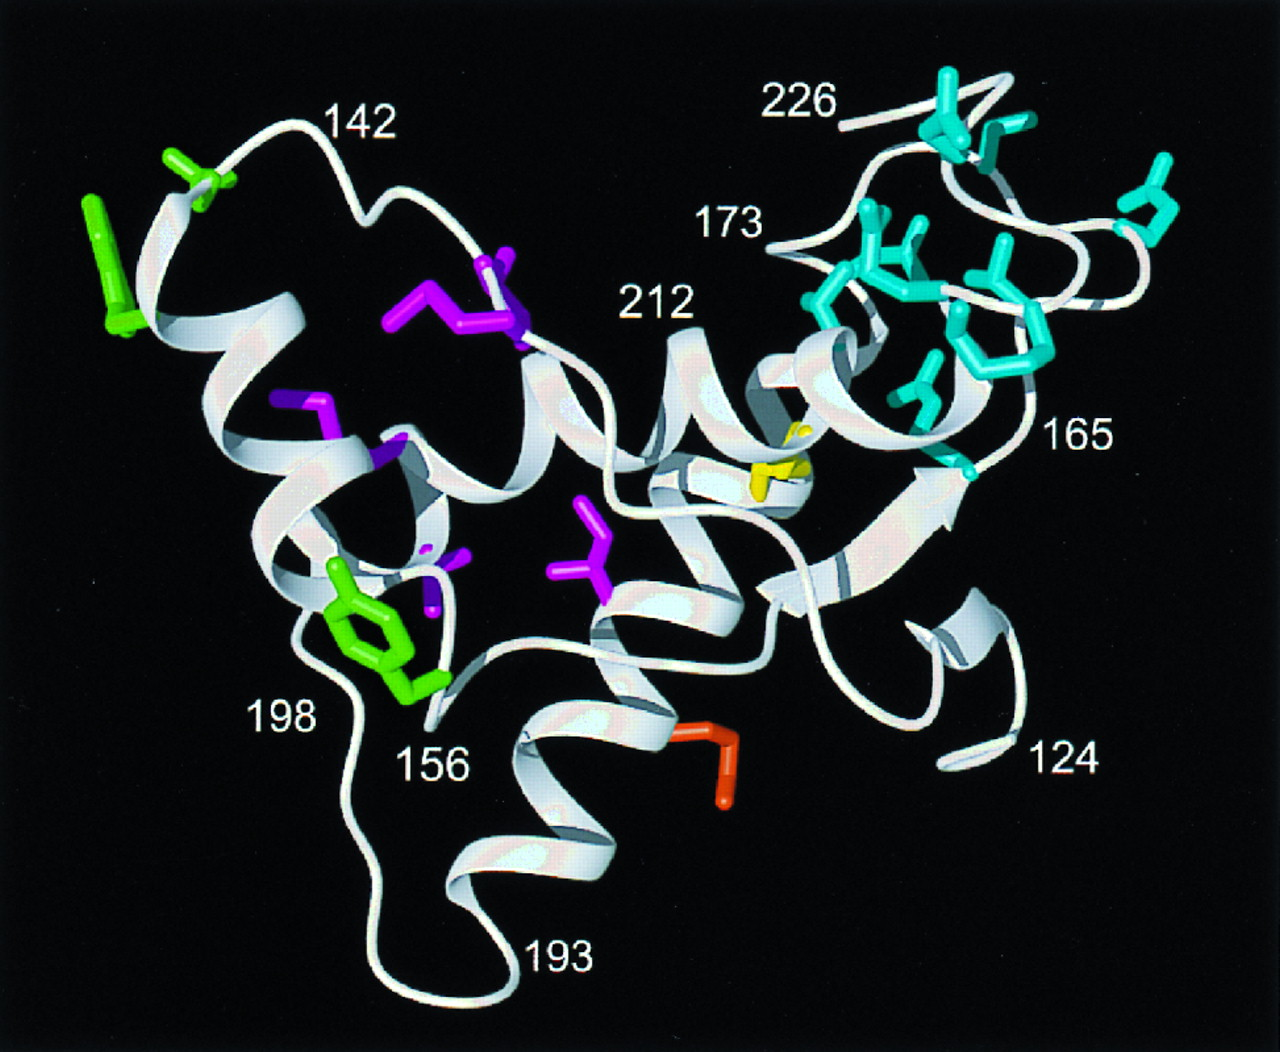
\includegraphics[width=\textwidth]{prion.jpg}
				\caption{NMR-derived structure of a prion  \url{http://www.pnas.org/content/94/14/7281.full}}
				\label{fig3}
			\end{minipage}					
		\end{figure}
	\end{frame}
	
	
	\begin{frame}{\thesection.\thesubsection. \insertsubsection}
		\begin{itemize}
			\item NMR relaxometry can be used to monitor molecular environment
		\end{itemize}

		\begin{figure}[ht]
					
						
			\begin{minipage}[t]{0.15\textwidth}
				\centering
				(a)
				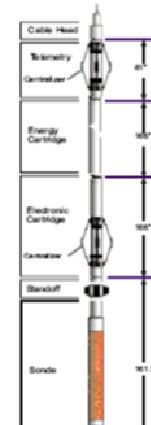
\includegraphics[width=\textwidth]{well_logging1.jpg}
			\end{minipage}
			\hspace{0.1cm}
			\begin{minipage}[t]{0.15\textwidth}
				\centering
				(b)
				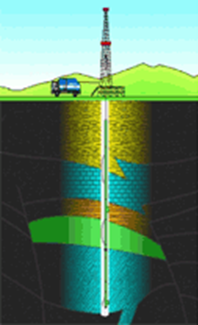
\includegraphics[width=\textwidth]{well_logging2.png}
				\label{fig7}
			\end{minipage}			
			\hspace{0.1cm}				
			\begin{minipage}[t]{0.15\textwidth}
				\centering
				(c)
				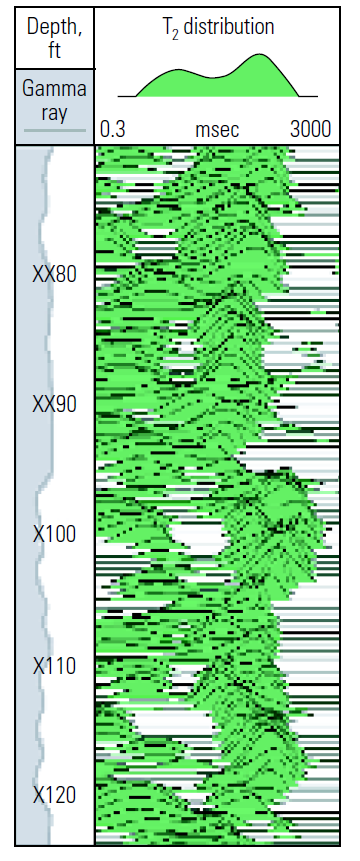
\includegraphics[width=\textwidth]{well_logging3.png}	
				\label{fig5}
			\end{minipage}		
			\hspace{0.1cm}
			\caption{ (a) NMR-logging probe, (b) Schematic positioning of the probe in a well, (c) T\textsubscript{2}-relaxation profile along the bore. Sources: 1) Allenet al. Oilfield review, Autumn 2000; 2) Coates, Xiao NMR Logging Principles and Applications, Hulliburton}		
		\end{figure}			
	\end{frame}
	
\begin{frame}{\thesection.\thesubsection. \insertsubsection}
	\begin{itemize}
		\item NMR forms the basis for magnetic resonance imaging (MRI)
	\end{itemize}
	
	\begin{figure}[ht]
			\centering
			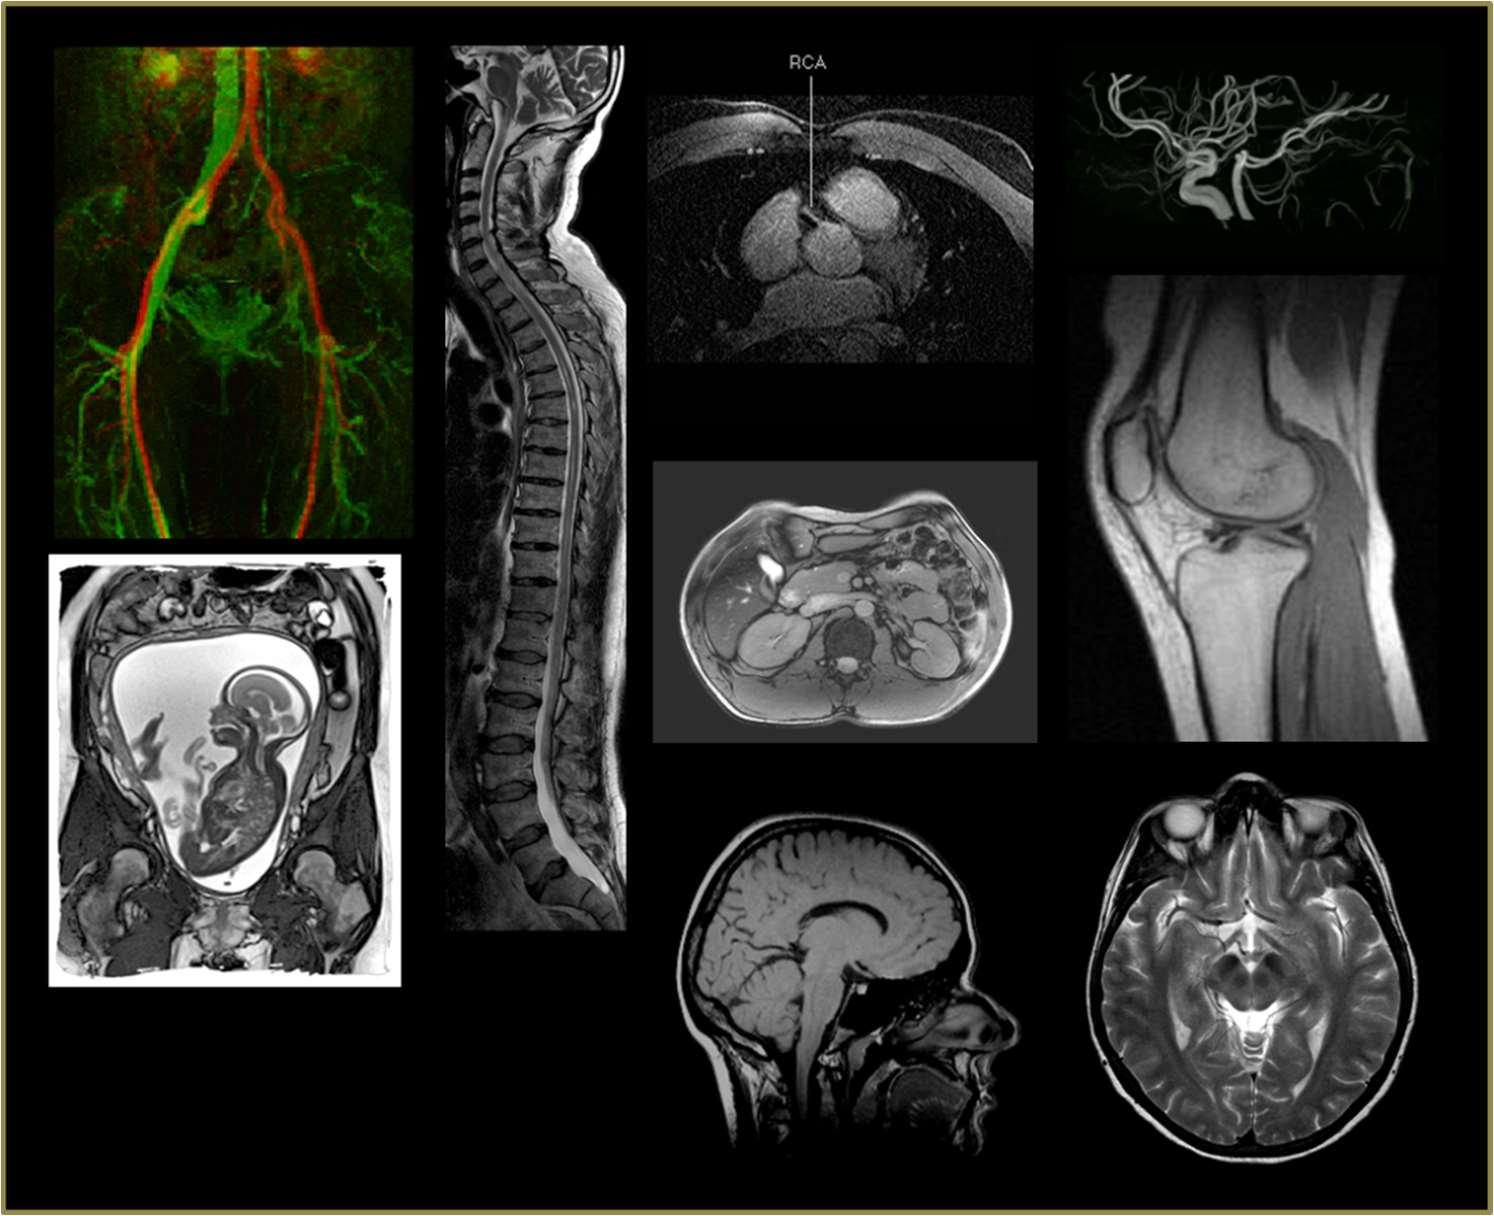
\includegraphics[width=0.7\textwidth]{mri.jpeg}
		\caption{  Example magnetic resonance images of blood vessel (in legs), fetus in utero, spine, heart, abdomen, head, blood vessels (in brain), knee, brain (courtesy of Prof. Richard Bowtell)}		
	\end{figure}			
\end{frame}


\subsection{Magnetic moments in magnetic field.}

\begin{frame}{\thesection.\thesubsection. \insertsubsection}
	
	\begin{itemize}[<+>]
		\item Consider charges moving in a limited volume. The position of a charge $\bm{e_n}$ will be given by a vector $\bm{r_n}$ and its velocity by $\bm{v_n}$. The overall magnetic moment of such a system is defined as:
			
			\begin{equation}
			\bm{M} = \frac{1}{2} \sum_{n} e_n\bm{r_n} \times \bm{v_n}
			\end{equation}
		\item 	If all the charges and masses are the same, then $\bm{M}$ can be rewritten as:	
			\begin{equation} \label{eq:1}
			\bm{M} = \frac{e}{2m} \sum_{n} m\bm{r_n} \times \bm{v_n} = \gamma \bm{L},
			\end{equation}
			where
			\begin{equation}
			\bm{L} = \sum_{n} \bm{p_n} \times \bm{r_n}
			\end{equation}
			is the mechanical angular momentum.
		\item 
			\alert{Gyromagnetic ratio}(or magnetogyric): 
			\begin{equation}
			\gamma = \dfrac{e}{2m}
			\end{equation}
			
	
	\end{itemize}
	


\end{frame}

\begin{frame}{\thesection.\thesubsection. \insertsubsection}
	\begin{itemize}[<+>]
		\item When a magnetic moment $\bm{M}$ is placed into an external uniform permanent magnetic field $\bm{B}$, its energy is given by:
			
			\begin{equation} \label{eq:2}
			E = -\bm{M} \cdot \bm{B}
			\end{equation} 
		\item  The torque acting on the system:
			\begin{equation}
			\frac{d\bm{L}}{dt} = \bm{M} \times \bm{B}
			\end{equation}
			  
		 \item  	Now using equation \ref{eq:1} we can obtain the equation describing the motion of vector $\bm{M}$:
			
			\begin{equation} \label{eq:precession_compact}
			\frac{d\bm{M}}{dt} = \gamma \bm{M} \times \bm{B}
			\end{equation}
			
	\end{itemize}
\end{frame}
\begin{frame}{\thesection.\thesubsection. \insertsubsection}
	\begin{itemize}[<+>]
		\item 
		    In a uniform magnetic field directed along $z$-axis $\bm{B} = (0, 0, B_0)$, the equation for individual components of $\bm{M}$ follow the equations:
		    
		    \begin{minipage}[b][4cm]{0.4\textwidth}
		    	\centering
		    	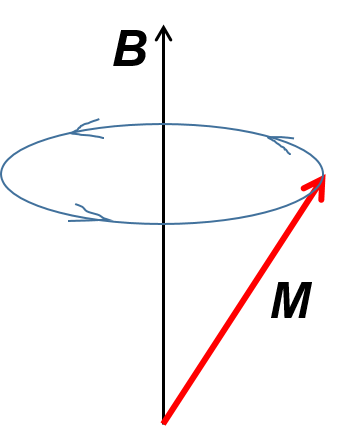
\includegraphics[width=0.7\textwidth]{precession.png}
		    \end{minipage}
		    \hspace{0.1cm}		    
		    \begin{minipage}[b][4cm]{0.4\textwidth}
		        \centering
		    	 \begin{equation} \label{precession}
		    	 \setlength{\jot}{5pt}
		    	 \begin{aligned}
		    	 \dfrac{dM_x}{dt} & =  \omega_L M_y \\
		    	 \dfrac{dM_y}{dt} & =  -\omega_L M_x \\
		    	 \dfrac{dM_z}{dt} & =  0,
		    	 \end{aligned}
		    	 \end{equation}
		    	 where $\omega_L = \gamma B_0$ - \alert{Larmor frequency}.
		    \end{minipage}
		    
		    
		\item
			A solution to this system of differential equations with initial values of $M_x(0), M_y(0), M_z(0)$ has the following form:
						
			\begin{equation} 
			\begin{array}{lcl}
			M_x(t) &=& M_x(0) \cos(\omega_L t) + M_y(0) \sin (\omega_L t) \\
			M_y(t) &=& -M_y(0) \sin(\omega_L t) + M_y(0) \cos (\omega_L t) \\
			M_z(t) &=& M_z(0) 
			\end{array}
			\end{equation}
		
		
	\end{itemize}
		
\end{frame}

\subsection{Angular momentum operator}
\begin{frame}{\thesection.\thesubsection. \insertsubsection}
	
	\begin{itemize}[<+>]
		\item     In quantum mechanics physical quantities $A$ are represented by their operators $\hat{A}$. The mechanical angular momentum is replaced by its corresponding operator:
		\begin{equation}
		\bm{L} = \sum_{n} \bm{p_n} \times \bm{r_n}  \longleftrightarrow \bm{\hat{L}} = \dfrac{1}{\hbar} \sum_{n} \bm{\hat{r}_n} \times \bm{\hat{p}_n} =   -i \sum_{n} \bm{\hat{r}_n} \times \bm{\nabla_n}
		\end{equation}
		\item Angular momentum operator properties. Commutation:
		\begin{equation}
		  [\hat{L}_y,\hat{L}_z] = i\hat{L}_x, [\hat{L}_z,\hat{L}_x] = i\hat{L}_y, [\hat{L}_x,\hat{L}_y] = i\hat{L}_z
    	\end{equation}
		\item Angular momentum squared, and its commutation properties:
        \begin{align}
          &\hat{L}^2 = \hat{L}_x^2 + \hat{L}_y^2 + \hat{L}_z^2 \\
          &[\hat{L}^2, \hat{L}_x^2]=[\hat{L}^2, \hat{L}_y^2]=[\hat{L}^2, \hat{L}_z^2]= 0       
        \end{align}        
	\end{itemize}

\end{frame}

\begin{frame}{\thesection.\thesubsection. \insertsubsection}
	\begin{itemize}[<+>]
		\item Eigenfunctions of both $\hat{L}^2$ and $\hat{L}_z$ operators can be characterized by integer quantum numbers $l$  and $m$ respectively. These eigen functions will be denoted as $\vert lm \rangle$. Their eigenvalues are:
		\begin{align}
		\hat{L}_z \vert lm \rangle &= m \vert lm \rangle \\
		\hat{L}^2 \vert lm \rangle &= l(l+1) \vert lm \rangle
		\end{align}
		\item Another useful operator are raising and lowering operators:
		\begin{align}
		  &\hat{L}_{+} = \hat{L}_x + i\hat{L}_y, \hat{L}_{-} = \hat{L}_x - i\hat{L}_y\\
		  &\langle lm \vert \hat{L}_{+} \vert l (m-1) \rangle = \langle l(m-1) \vert \hat{L}_{-} \vert lm \rangle = \sqrt{(l+m)(l-m+1)}
		\end{align}
	\end{itemize}
	
\end{frame}


\begin{frame}{\thesection.\thesubsection. \insertsubsection}
	\begin{itemize}[<+>]
		\item
			Classical magnetic moment will have its own quantum analogue, the operator of angular momentum:
			\begin{equation}
			\bm{M} = \gamma \bm{L}  \longleftrightarrow \bm{\hat{\mu}} = \gamma \hbar \bm{\hat{L}}
			\end{equation} 
		\item Bohr magneton:
		\begin{equation}
			\beta = \dfrac{e\hbar}{2m} \approx 9.27 \cdot 10^{-24}  \text{J T}^{-1}
		\end{equation}
	\end{itemize}

\end{frame}


\begin{frame}{\thesection.\thesubsection. \insertsubsection}
	Free electron and many nuclei have spin. 
\end{frame}


\begin{frame}

	These equations describe a precession of a vector $\bm{M}$ around the direction of the external magnetic field $\bm{B}$ with the frequency $\omega_0$ as shown schematically in Fig.\ref{fig:precession}A. Such motion is called  "Larmor precession" and $\omega_0 = \gamma B_0$ is called "Larmor frequency".
	
	Of course, this primitive classical picture serves only as an illustration to the actual behaviour of magnetic moments placed into a magnetic field. However, a more rigorous description using quantum mechanics for an ensemble of magnetic moments provides a similar answer. Larmor precession of an overall magnetic moment is a real effect, and as we will see later, it is essential for acquiring of magnetic resonance spectra.
	

	
	Now we'll briefly sketch the basic quantum mechanical description of a magnetic moment in a magnetic field.  The angular momentum operator $\bm{\hat{L}}$ (which could be an orbital or spin angular momentum) is proportional to the magnetic moment operator as:
	\begin{equation} \label{eq:3}
	\bm{\hat{\mu}} = \gamma \hbar \bm{\hat{L}},
	\end{equation}
	The Hamiltonian of a system can be written by analogy with expression \ref{eq:2} as:
	\begin{equation} \label{eq:2level}
	\hat{H} = -\bm{\hat{\mu}} \bm{B} = -\gamma \hbar \hat{I}_{z} B_0 = -\omega_0 \hat{I}_{z},
	\end{equation}
	
	The level diagram in Fig.\ref{fig:precession}B shows schematically the splitting of $\gamma \hbar B_0 $ between energy levels  as a function of the applied magnetic field for a system with only a spin-$\frac{1}{2}$ angular momentum. In this case, the eigenfunctions corresponding to the two energy levels are just the two projections of a spin onto the $z$-axis: $m_z=+\frac{1}{2}$ is $\vert \alpha \rangle$ and $m_z=-\frac{1}{2}$ is $\vert \beta \rangle$.
	
	
\end{frame}

\end{document}